When the string is plucked, it will create travelling waves on the string that reflect at both ends, creating standing waves. The frequency of the standing waves with the longest wavelength is the fundamental frequency, also called the first harmonic. This is the lowest frequency, and there will usually be other higher harmonics that when combined create the characteristic timbre of the electric guitar.

%\begin{figure}[h]
%    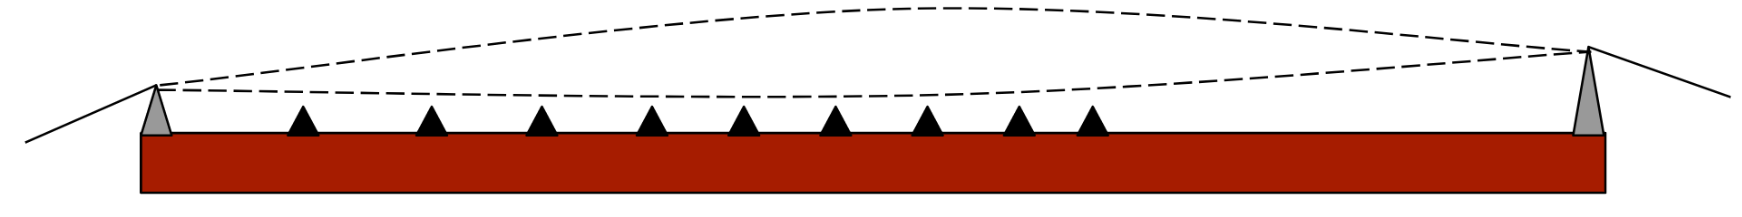
\includegraphics[width=\textwidth]{./ee/fig2.png}
%    \caption{The “open” string (not fretted) is plucked and vibrating at its fundamental frequency.}\label{fig2}
%\end{figure} 
The fundamental frequency $f_0$ of a string can be determined by Mersenne's law:
\begin{equation}\label{eqn1}
    f_0 = \frac{1}{2l_s}\sqrt{\frac{T}{\mu}}
\end{equation}
where $l_s$ is the vibrating length of the string, $T$ is the tension, and $\mu$ is the linear density of the string (mass of string per unit length). \cite{mersenne} \par
%From Figure \ref{fig2} we see the wavelength is double the length of the guitar - the “scale length” $l$ . Therefore \begin{equation}\label{eqn2}
%    \lambda = 2l
%\end{equation}
%The speed of the wave $v$ on a stretched string with tension $T$ can be determined by the equation:
%\begin{equation}\label{eqn3}
%    v = \sqrt{\frac{T}{\mu}} 
%\end{equation}
%Where $\mu$ is the linear density of the string (mass of string per unit length) \cite{eqn3}\par
%Substitute (\ref{eqn2}) and (\ref{eqn3}) into (\ref{eqn1}) we get the expression for the frequency of an open string
%\begin{equation}\label{eqn4}
%    f_0 = \frac{1}{2l}\sqrt{\frac{T}{\mu}}
%\end{equation}
When the string is pressed down on a fret and plucked, its vibrating length changes, changing the frequency. Figure \ref{fig2} shows a model of the string pressed down on fret $n$. The distance from the bridge to the fret then is $l_n$

\begin{figure}[!htbp]
    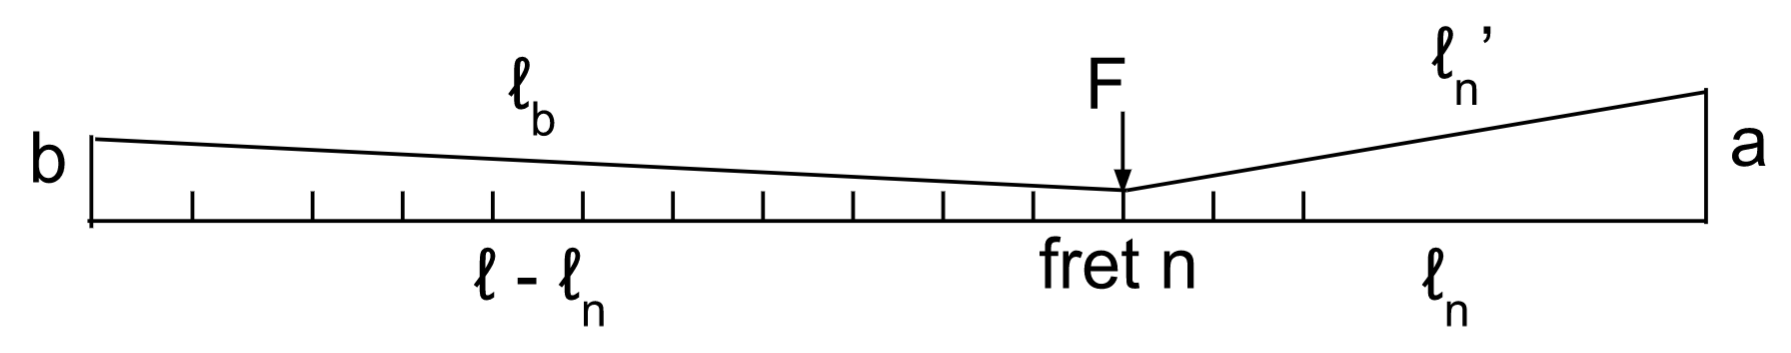
\includegraphics[width=\textwidth]{./ee/fig3.png}
    \caption{A simplified model of the fretted string}\label{fig2}
\end{figure} 
%Theoretically, the frequency of this note is 
%\begin{equation}\label{eqn5}
%    f_n = \frac{1}{2l_n}\sqrt{\frac{T}{\mu}}
%\end{equation}
In Western music, the ubiquitous musical system is the twelve-tone equal temperament (12-TET) system, where an octave is divided into 12 equally spaced notes on a logarithmic scale \cite{yuval}. The ratio is thus equal to $\sqrt[12]{2}$, therefore to position the frets correlating to the notes, the scale length needs to be divided into powers of $\sqrt[12]{2}$. To do this, luthiers traditionally use a formula to calculate the position of each fret. \cite{eqn6}
\begin{equation}\label{eqn2}
    l_n=\frac{l}{2^\frac{n}{12}}
\end{equation}